%!TEX TS-program = xelatex
%!TEX encoding = UTF-8 Unicode

%%%  Syllabus template for use with style files at http://kjhealy.github.com/latex-custom-kjh
%%%  Kieran Healy

\documentclass[11pt,article,oneside]{memoir}

% packages
\usepackage{org-preamble-xelatex}
\usepackage{wallpaper}
\usepackage{xcolor}
\usepackage[super]{nth}
\usepackage[inline]{enumitem}
\usepackage{moreenum}
\usepackage{tabu}
\usepackage{booktabs}
\AtBeginBibliography{\small}

% Definitions
\def\myauthor{Author}
\def\mytitle{Title}
\def\mycopyright{\myauthor}
\def\mykeywords{}
\def\mybibliostyle{plain}
\def\mybibliocommand{}
\def\mysubtitle{}
\def\myaffiliation{Louisiana State University}
\def\myaddress{309 Design}
\def\myemail{baharmon@lsu.edu} 
\def\myweb{https://baharmon.github.io/}
\def\myphone{919.622.8414}
\def\myversion{}
\def\myrevision{}
\def\myaffiliation{\ \\Louisiana State University}
\def\myauthor{Brendan Harmon}
\def\mykeywords{Landscape Architecture}
\def\mytitle{Participatory modeling for Jean Lafitte \newline}
\def\mysubtitle{\large \textbf{Coastal Sustainability Studio |} \normalfont Community Project Proposal}

% color
\makeatletter
\newcommand{\globalcolor}[1]{%
  \color{#1}\global\let\default@color\current@color
}
\makeatother

% begin
\begin{document}

\setlength\bibitemsep{0.75em}

% fonts
\defaultfontfeatures{}
\defaultfontfeatures{Scale=MatchLowercase}         
\setmainfont[Scale=1, Path = fonts/lato/,BoldItalicFont=Lato-RegIta,BoldFont=Lato-Reg,ItalicFont=Lato-LigIta]{Lato-Lig}
\setsansfont[Scale=1, Path = fonts/lato/,BoldItalicFont=Lato-RegIta,BoldFont=Lato-Reg,ItalicFont=Lato-LigIta]{Lato-Lig}
\setmonofont[Mapping=tex-text,Scale=0.8,Path = fonts/inconsolata/]{i}

\def\ind{\hangindent=1 true cm\hangafter=1 \noindent}
\def\labelitemi{$\cdot$}
\chapterstyle{article-4-sans}  
\title{\LARGE \mytitle \newline \mysubtitle}     
\author{\Large\myauthor \newline \footnotesize\texttt{\noindent\myemail}}
%\date{Spring 2018. Design 217.\newline Monday, Wednesday, \& Friday 9:30am--11:30am.}
%\published{\,}
\date{}
% -------------------------------- BODY -------------------------------- 

\pagenumbering{arabic}
\globalcolor{black}
\vspace*{-10em}
\maketitle

\vspace*{-3em}


% -------------------------------- FIGURE -------------------------------- 

\begin{figure}
    \begin{center}
        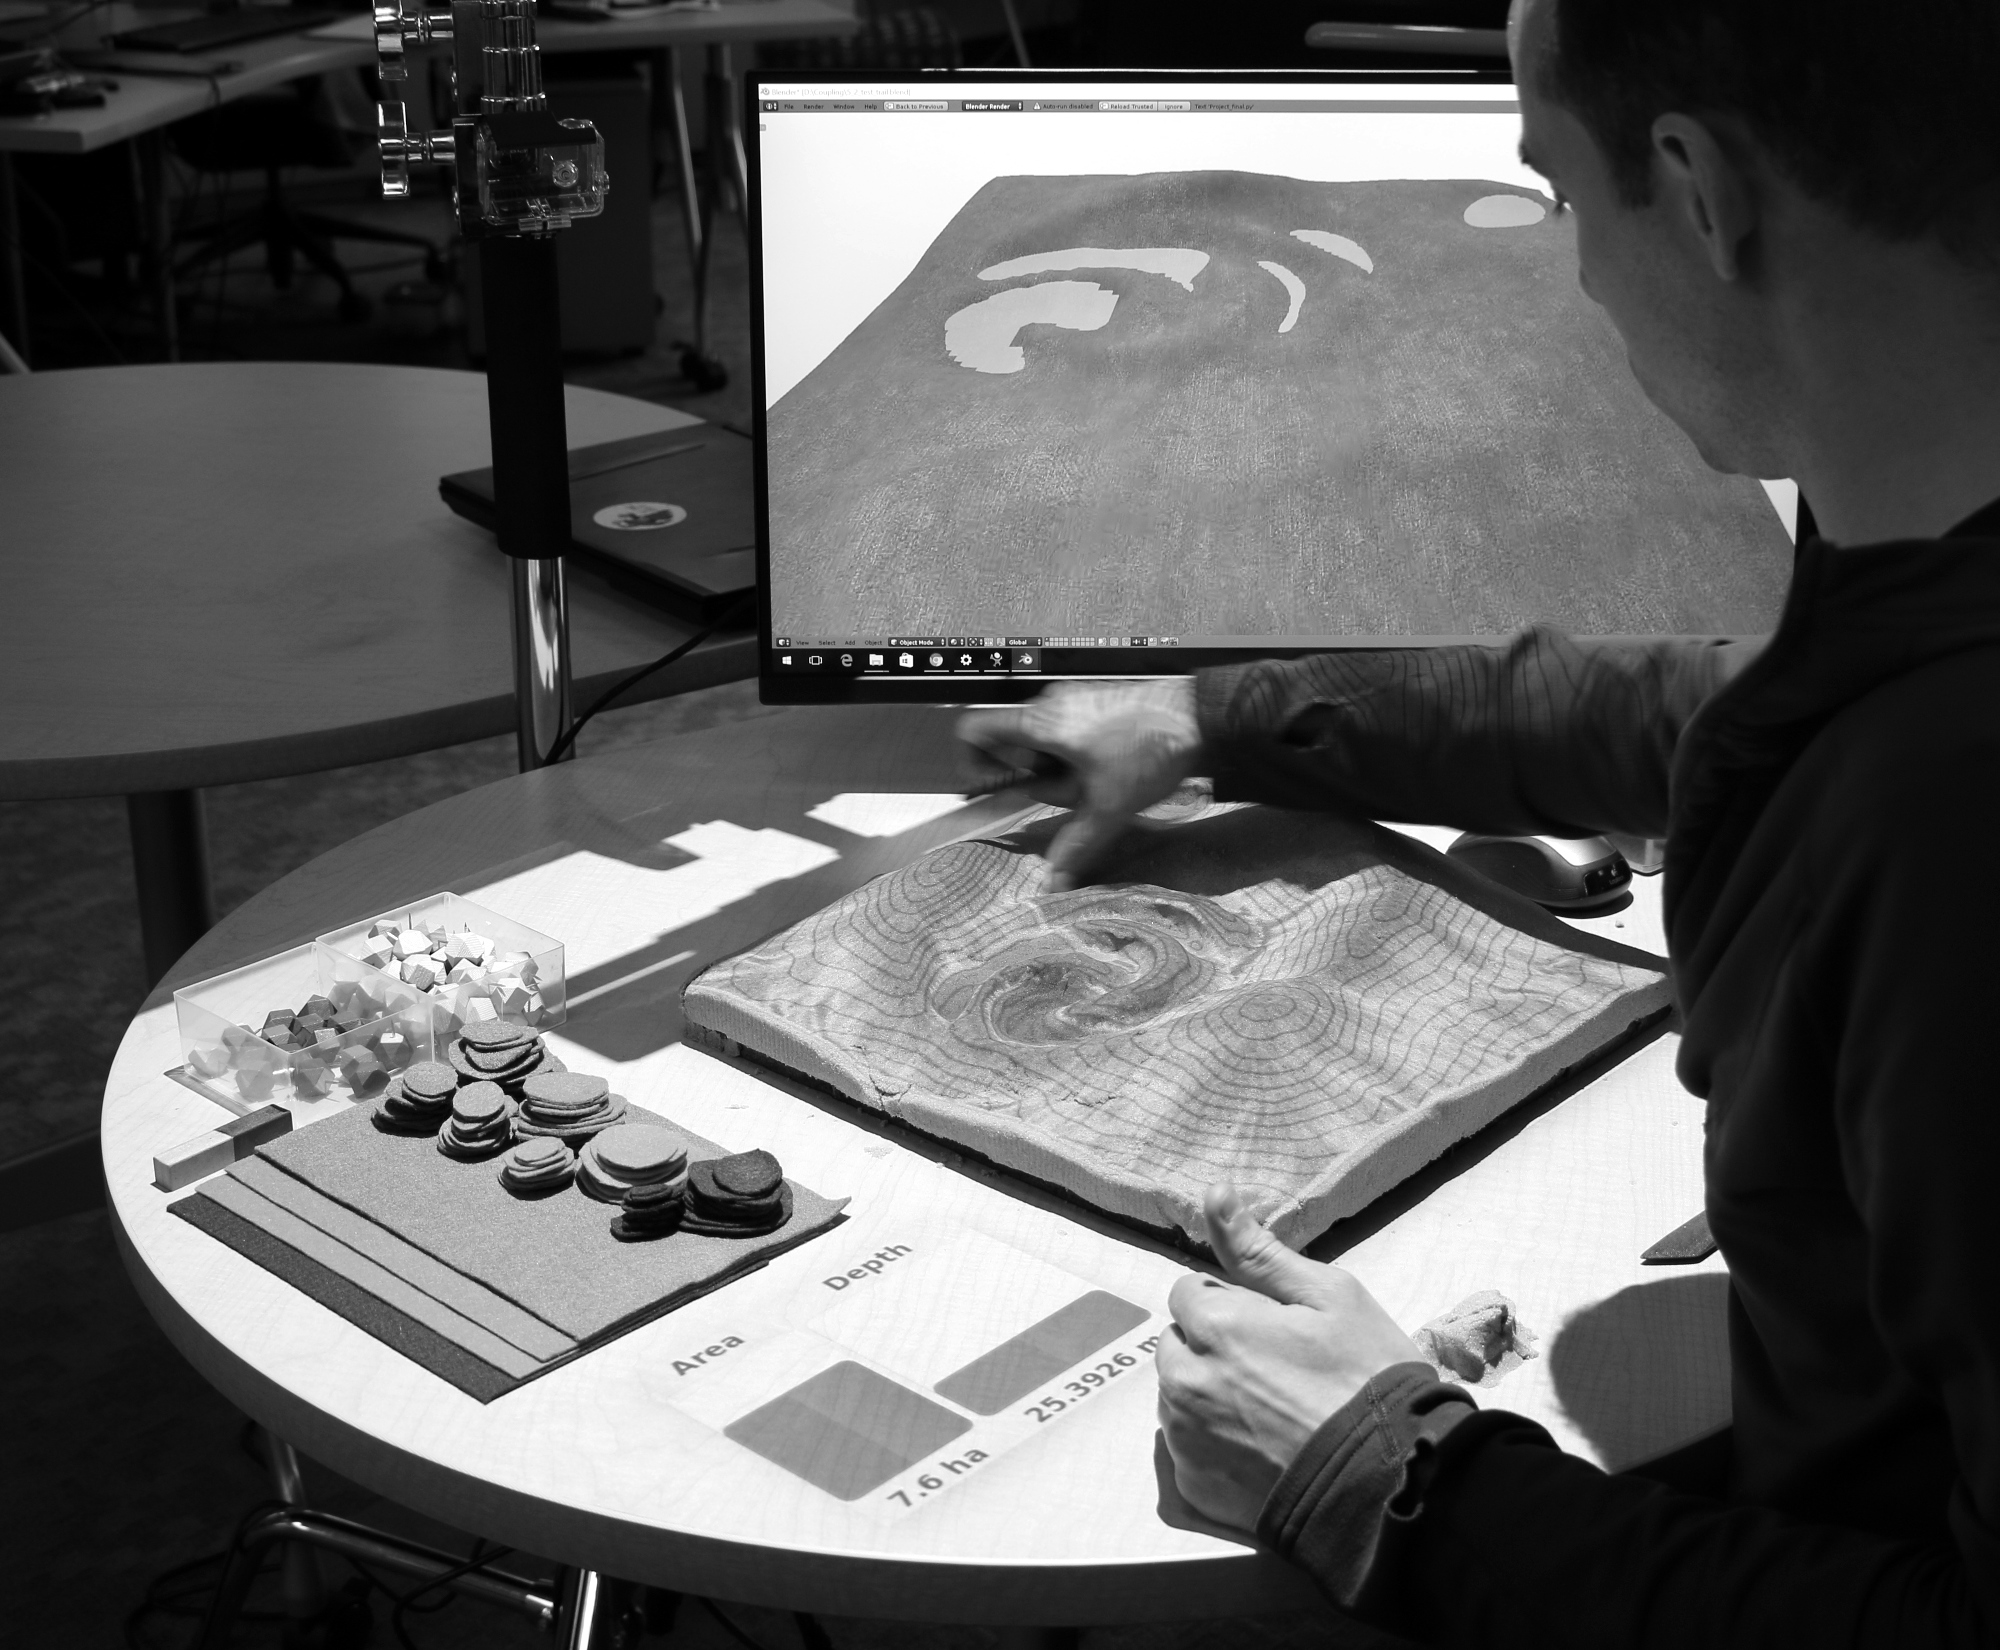
\includegraphics[width=0.45\textwidth]{../images/sculpting_4_grey.jpg}
        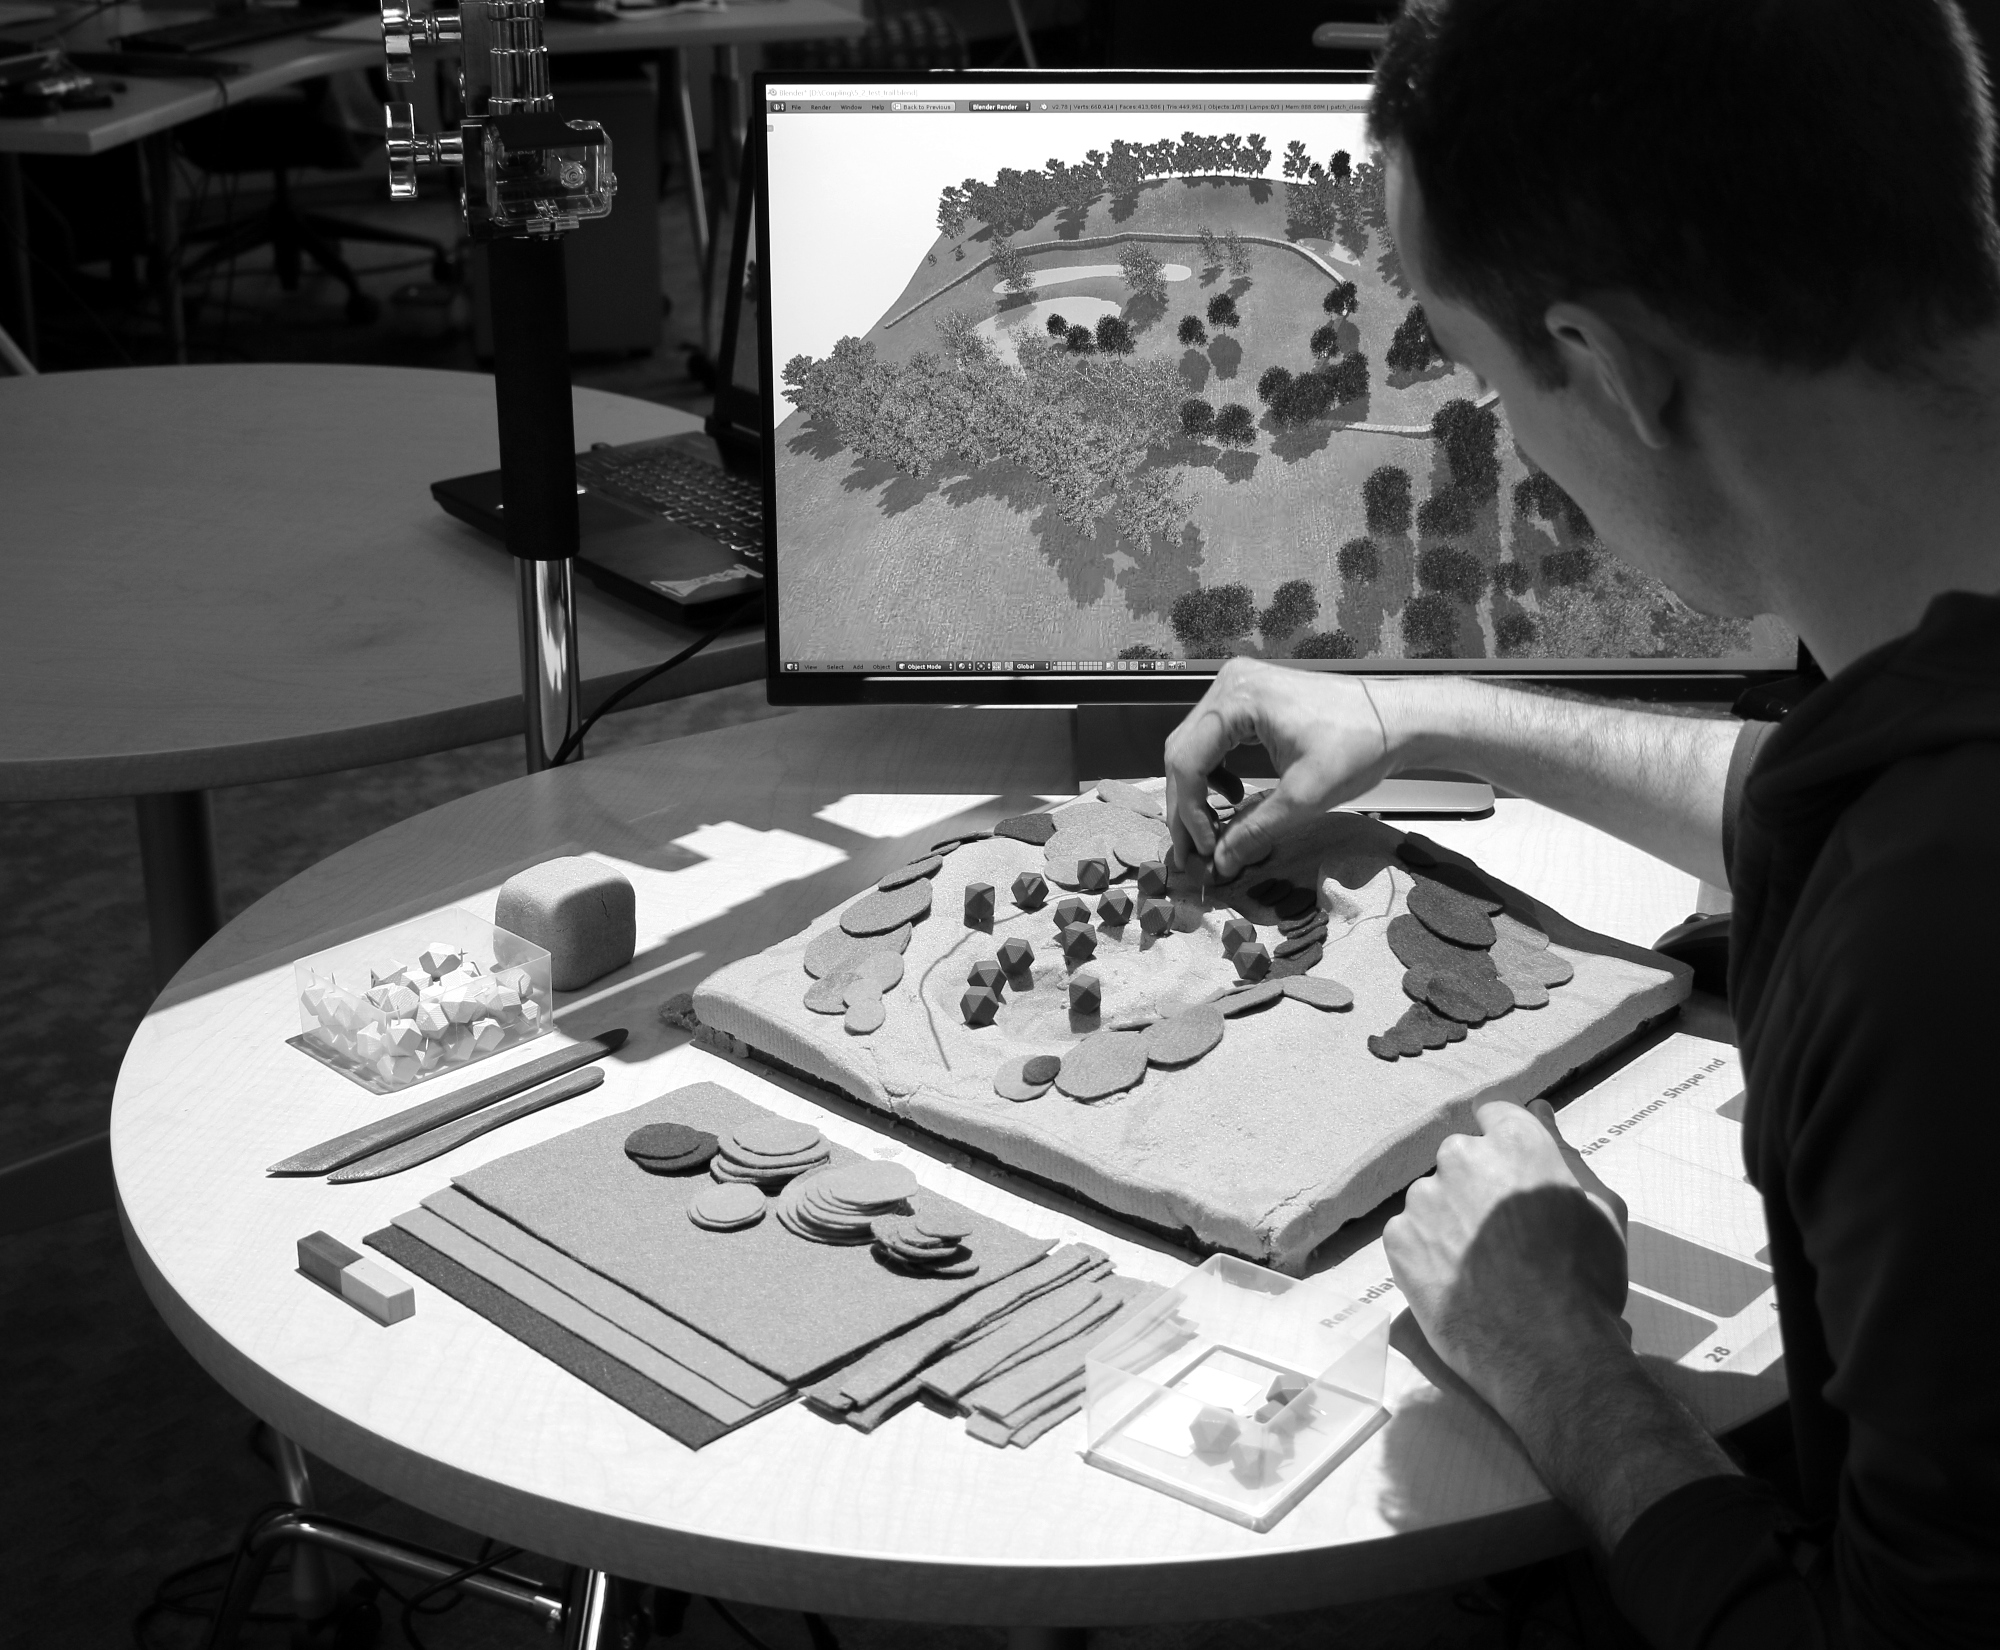
\includegraphics[width=0.45\textwidth]{../images/specimen_planting_3_grey.jpg}
        \caption{Tangible Landscape: a real-time cycle of 3D scanning, geospatial computation and 3D modeling, and projection and 3D rendering.}
        \label{fig:diagram}
    \end{center}
\end{figure}

%\begin{figure}
%    \begin{center}
%        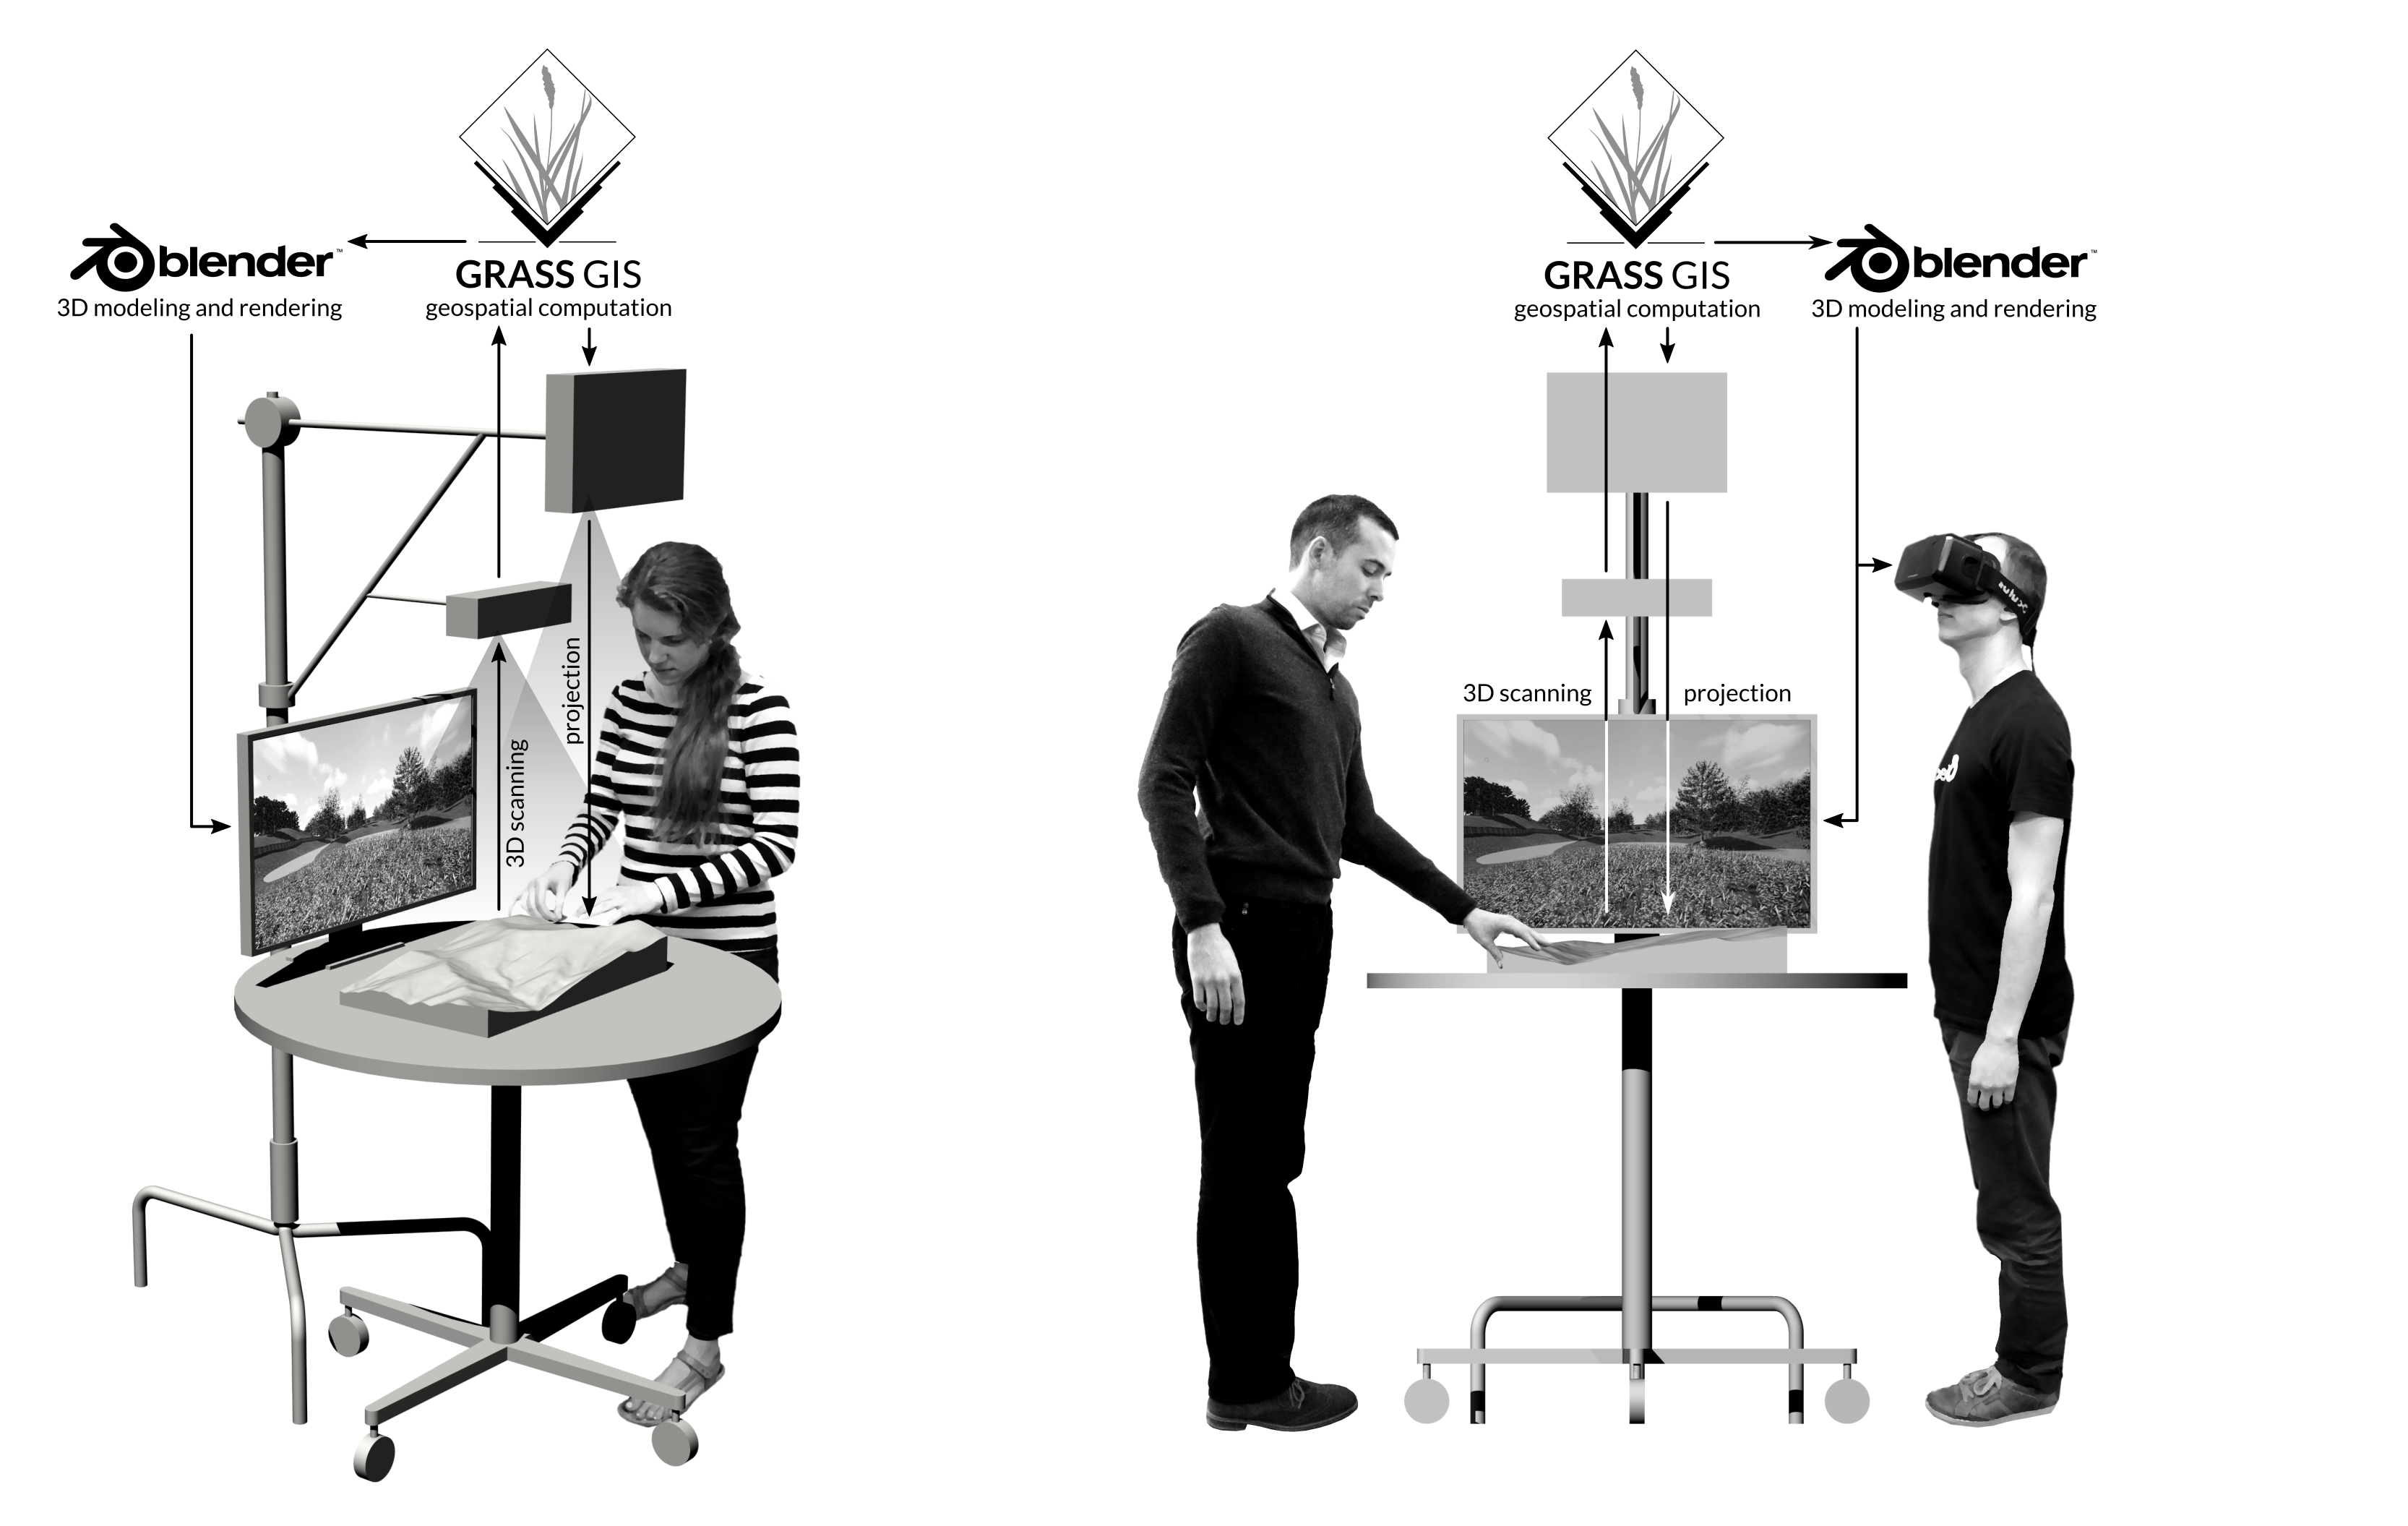
\includegraphics[width=\textwidth]{../images/rendered_diagram_1.png}
%        \caption{Tangible Landscape: a real-time cycle of 3D scanning, geospatial computation and 3D modeling, and projection and 3D rendering.}
%        \label{fig:diagram}
%    \end{center}
%\end{figure}

% -------------------------------- DESCRIPTION -------------------------------- 

\noindent \textbf{Project description}
I propose running a participatory modeling studio 
with the \nth{3} year graduate landscape architecture class
to collaboratively model and visualize alternative futures 
for the town of Jean Lafitte in Jefferson Parish, Louisiana.   
%
The studio would address 
the impact of coastal change 
-- of storm surge, flooding, erosion, and land-loss --
on Jean Lafitte.
%
In collaboration with Louisiana Sea Grant 
%\url{http://www.laseagrant.org/}
we would hold a series of participatory workshops 
in the community.
%
Using geospatial modeling, tangible interaction, and virtual reality
the students would work with community members to develop 
their own plans for adapting to and living with coastal change.
%
As a thesis project
another landscape architecture graduate student
would use cognitive mapping 
to study the community's relationship with their environment
and the impacts of coastal change.
%
The goal of this studio and research 
would be to help community members 
map and document their cultural heritage,
model scenarios,
and develop and visualize plans
for adapting to coastal change, 
while conserving vernacular heritage. 
%
At the end of the studio we will showcase 
the process and results in a report, exhibition, 
and website. \\

% -------------------------- RESEARCH METHODS ----------------------------
\noindent \textbf{Methods}
As research the aim of this project is to
study how tangible interfaces for geospatial modeling
can be used for participatory modeling, planning, and design.
%
We will use Tangible Landscape 
-- an open source system that interactively couples 
a physical model and digital model of a landscape in real-time --
in participatory modeling workshops
so that students and community members 
can intuitively, collaboratively model new landforms, planting, routes, and structures
and see how these change geospatial analyses and simulations 
like water flow, erosion, and flooding
in real-time (Fig.~\ref{fig:diagram}). 
% 
See \url{http://tangible-landscape.github.io/}
%and \url{https://youtu.be/pYbpEMjME1Y} 
to learn more about Tangible Landscape.
%
We will also use digitally fabricated models, 
360 degree photography and video, 
and virtual reality as tools 
to help the community visualize 
how their dynamic environment may change. 
%
Our objectives are to
\begin{enumerate*}[label=\alph*),font=\itshape]
\item intuitively visualize scientific analyses and models of coastal change,
\item engage community stakeholders in modeling and planning 
through tangible interaction and immersive visualization,
and
\item develop a case study for participatory modeling with Tangible Landscape.
\end{enumerate*} \\

% -------------------------------- TEAM -------------------------------- 
\noindent \textbf{Team}
%
\begin{table}[H]
\small
\begin{tabu} to \textwidth {lX}
\toprule
Role & Name\\
\midrule
PI \& Instructor & Brendan Harmon \\
MLA Thesis Student & Philip Fernberg \\
Visiting researchers & Anna Petrasova \& Payam Tabrizian \\
Collaborators & Matt Bethel at LA Sea Grant \\
\bottomrule
\end{tabu}
\end{table}

% ------------------------- DELIVERABLES ------------------------ 

\noindent \textbf{Deliverables}
%
\begin{table}[H]
\small
\begin{tabu} to \textwidth {lX}
\toprule
Deliverable & Topic\\
\midrule
Report for CSS & Participatory modeling for Jean Lafitte\\
Paper & Participatory modeling with Tangible Landscape\\
Thesis & Cognitive mapping of Jean Lafitte\\
Website \& video & Record of the participatory process\\
Exhibition & Showcase the participatory process and its results\\
\bottomrule
\end{tabu}
\end{table}

% -------------------------------- BUDGET -------------------------------- 
\noindent \textbf{Budget}
%
\begin{table}[H]
\small
\begin{tabu} to \textwidth {lXr}
\toprule
Category & Item & Cost\\
\midrule
Tangible Landscape & Parts \& materials & \$1500 \\
Digital fabrication & Materials & \$1300 \\
360 Photography & Ricoh Theta V & \$500 \\
Publication & Report writing \& printing & \$1200 \\
Exhibition & Materials \& setup & \$500 \\
Travel & Van rental \& airfare for visiting researchers & \$1000 \\
& \textbf{Total} & \textbf{\$6,000}\\
\bottomrule
\end{tabu}
\end{table}

\end{document}
